\chapter{Algoritmus pro analýzu dynamických systémů}\label{chapter:algorithm}

Tato kapitola ukáže jednu z možností, jak přistoupit k analýze modelů zadaných
pomocí obyčejných diferenciálních rovnic. Zde uvedená analýza se snaží řešit následující
problémy:
\begin{enumerate}
	\item\label{item:init}	Máme k dispozici již hotový model, jehož chování odpovídá chování skutečného
			systému pro jedno konkrétní nastavení iniciálních hodnot stavovým
			proměnným. Splňuje tento model požadované vlastnosti i~pro jiná nastavení?
	\item	Máme kostru modelu, v němž se vyskytuje několik parametrů, jejichž hodnota
			není známá. Jak nastavit parametry modelu tak, aby splňoval dané chování~\cite{aster2012}?
\end{enumerate}

V~bodě \ref{item:init} lze jít dál než k pouhé kontrole modelů. Můžeme si představit
poměrně přesný model, který využijeme k analýze jeho chování v~pod\-mín\-kách, které nelze
navodit u reálného systému. Typickým příkladem může být živý organismus v~toxickém
prostředí nebo extrémně vysoká nákaza šířící se ce\-lo\-svě\-to\-vou populací.

\section{Definice problému}\label{section:initial:condtion:problem:definition}

Nechť je dynamický systém $\mathcal{DS} = (\mathbf{X}, f(\mathbf{P}))$, kde $\mathbf{X} = (x_1, \ldots, x_n) \in \mathbb{R}^n$
je vektor stavových proměnných a $\mathbf{P}  = (p_1, \ldots, p_m) \in \mathbb{R}^m$ je vektor parametrů. Dynamiku systému popisují obyčejné diferenciální
rovnice $\frac{dx_i}{dt} = f_i(\mathbf{P})(\mathbf{X})$ a $f_i: \mathbb{R}^m \rightarrow (\mathbb{R}^n \rightarrow \mathbb{R}^n)$.
Tento systém rovnic souhrnně označíme jednou rovnicí $\frac{d\mathbf{X}}{dt} = f(\mathbf{P})(\mathbf{X})$. Na rozdíl
od obecného modelu zadaného pomocí systému obyčejných diferenciálních rovnic uvažujeme pouze autonomní systémy,
tedy budeme předpokládat, že funkce stojící na pravé straně ne\-zá\-vi\-sí na čase, a proto je čas z definicí funkcí zcela vynechán.

Pro každou stavovou proměnnou $x_i$ je dán interval $\mathcal{I}_{x_i} = [\iota_{x_i}^{min}, \iota_{x_i}^{max}]$
a pro každý parametr $p_j$ interval $\mathcal{I}_{p_j} = [\iota_{p_j}^{min}, \iota_{p_j}^{max}]$.
Tyto intervaly omezují nastavení iniciálních hodnot stavových proměnných $x_i$, respektive o\-hod\-no\-ce\-ní
parametrů $p_j$, a určují tak prostor iniciálních podmínek \cite[str. 23]{drazan2011}.

\begin{align}
\mathcal{I} &= \mathcal{I}_{x_1} \times \mathcal{I}_{x_n} \times \ldots \times \mathcal{I}_{p_1} \times \ldots \times \mathcal{I}_{p_m}
\end{align}

Pro vektor $\mathbf{V} = (x_1, \ldots, x_n, p_1, \ldots, p_m) \in \mathcal{I}$ definujme projekční funkce $\pi_x(\mathbf{V}) = (x_1, \ldots, x_n)$
a $\pi_p(\mathbf{V}) = (p_1, \ldots, p_m)$. Je-li dána numerická metoda $\mathcal{M}_\varepsilon$,
formule temporální logiky signálů $\varphi$, dynamický systém $\mathcal{DS}$
a prostor iniciálních podmínek $\mathcal{I}$, pak řešeným problémem je najít
části prostoru $\mathcal{S}, \mathcal{N} \subseteq \mathcal{I}$ takové, že platí
vztah \ref{eq:initial:value:problem} \cite[str. 23]{drazan2011}.

\begin{align}\label{eq:initial:value:problem}
\begin{array}{ll}
\forall \mathbf{V} \in \mathcal{S} . \mathcal{M}^\tau_\varepsilon(f(\mathbf{P}), \mathbf{X}, \Delta t) \models \varphi, \textrm{~kde~} \mathbf{P} = \pi_p(\mathbf{V}), \mathbf{X} = \pi_x(\mathbf{V}) \\
\forall \mathbf{V} \in \mathcal{N} . \mathcal{M}^\tau_\varepsilon(f(\mathbf{P}), \mathbf{X}, \Delta t) \not\models \varphi, \textrm{~kde~} \mathbf{P} = \pi_p(\mathbf{V}), \mathbf{X} = \pi_x(\mathbf{V})
\end{array}
\end{align}

Tyto části prostoru popisují ohodnocení počátečních stavů a parametrů, za kterých se daný systém vyvíjí
s požadovanou vlastností $\varphi$, respektive bez po\-ža\-do\-vané vlastnosti. Naivní algoritmus řešící
tento problém do prostoru iniciálních podmínek vloží určité množství bodů a tyto body
použije pro simulaci chování modelu, nad kterým se následně provede ověření vlastnosti.
Počet bodů, tedy míra zahuštění prostoru iniciálních podmínek, závisí na požadované přesnosti
analýzy. I přes nesporné výhody tohoto přístupu snadno narazíme na výpočetní limity
potřebného množství bodů, a proto je vhodné pokusit se počet bodů omezit.


\section{Původní algoritmus}

Původní algoritmus, na kterém staví tato práce vychází z velice důležitého předpokladu:
\uv{Většina řešení začínajících v iniciálních bodech blízko sebe zůstávají blízko sebe
i v průběhu času~\cite[str. 25]{drazan2011}.} Předpokládá se tedy, že chování určená blízkými
hodnotami z prostoru iniciálních podmínek mají i blízkou míru platnosti dané formule.
Není tedy třeba zjišťovat chování pro všechny body prostoru iniciálních podmínek,
ale jen pro určitou množinu reprezentantů, pro kterou platí \cite[str. 25]{drazan2011}:

\begin{enumerate}
	\item	Chování blízké reprezentantovi zůstane blízké na celém časovém intervalu,
			na kterém je daná formule ověřována.
	\item	Množina reprezentantů pokrývá celý prostor iniciálních podmínek.
\end{enumerate}

Algoritmus do prostoru iniciálních podmínek vkládá body tak dlouho, dokud si trajektorie chování
určených blízkými body jsou vzdálenější než daná vzdálenost $\delta$. Nad simulovanými chováními
se ověří platnost formule. Výsledkem je určité množství bodů, u kterých dostáváme informace,
zda z nich simulovaná chování splňují či nesplňují danou vlastnost. Tyto body nastíní
hranice regionů platnosti a neplatnosti se zvolenou přes\-nos\-tí~$\delta$.

\begin{algorithm}
\caption{Analýza prostoru iniciálních podmínek}
\label{algorithm:main:original}
\begin{algorithmic}[1]
\Require 	$\mathcal{DS} = (\mathbf{X}, f), \mathcal{I}, \varphi, \Delta t, \delta, \varepsilon$
\Ensure 	$\textsc{Result} = \{([\mathbf{F}_0]_0, s_1), \ldots ([\mathbf{F}_k]_0, s_k)\}$ \Comment body a splněnost $\varphi$
\State		$\textsc{M}_{new} 	\gets $ počáteční zahuštění $\mathcal{I}$
\State		$\textsc{Result} \gets \emptyset$
\While{$\textsc{M}_{new} \neq \emptyset$}
	\State $\textsc{M}_{old} \gets \textsc{M}_{new}, \textsc{M}_{new} \gets \emptyset$
	\For{$([\mathbf{X}_{main}]_0, [\mathbf{P}_{main}]) \in \textsc{M}_{old}$}
		\State $\textsc{Traj}_{main} \gets \mathcal{M}^{||\varphi||}_\varepsilon(f_{\mathbf{P} \gets [\mathbf{P}_{main}]}, [\mathbf{X}_{main}]_0, \Delta t)$
		\State $\textsc{Satisfied}_{main} \gets $ splněnost $\varphi$ nad $\textsc{Traj}_{main}$
		\State $\textsc{Result} \gets \textsc{Result} \cup \{(\textsc{Satisfied}_{main}, [\mathbf{X}_{main}]_0, [\mathbf{P}_{main}])\}$
		\State $\textsc{Neigh} \gets $ body sousedící s bodem $([\mathbf{X}]_0, [\mathbf{P}])$
		\For{$([\mathbf{X}_{neigh}]_0, [\textbf{P}_{neigh}]) \in \textsc{Neigh}$}
			\State $\textsc{Traj}_{neigh} \gets \mathcal{M}^{||\varphi||}_\varepsilon(f_{\mathbf{P} \gets [\mathbf{P}_{neigh}]}, [\mathbf{X}_{neigh}]_0, \Delta t)$
			\State $\textsc{Satisfied}_{neigh} \gets $ splněnost $\varphi$ nad $\textsc{Traj}_{neigh}$
			\State $\textsc{Result} \gets \textsc{Result} \cup \{(\textsc{Satisfied}_{main}, [\mathbf{X}_{main}]_0, [\mathbf{P}_{main}])\}$
			\State $\textsc{Distance} \gets $ vzdálenost $\textsc{Traj}_{main}$ a $\textsc{Traj}_{neigh}$\label{algorithm:line:trajectory:distance}
			\If{$\textsc{Distance} > \delta$}\label{algorithm:line:trajectory:delta}
				\State	$\textsc{M}_{new} \gets \textsc{M}_{new} \cup \{(\frac{[\mathbf{X}_{main}]_0 + [\mathbf{X}_{neigh}]_0}{2}, \frac{[\mathbf{P}_{main}] + [\mathbf{P}_{neigh}]}{2})\}$
			\EndIf
		\EndFor
	\EndFor
\EndWhile
\end{algorithmic}
\end{algorithm}

Je samozřejmé otázkou, jakým způsobem konkrétně probíhá počáteční zahuštění prostoru
iniciálních podmínek, co přesně obsahuje mno\-žina sousedů daného bodu a jak
se změří vzdálenost dvou chování. Poslední zmí\-ně\-nou otázkou se podrobně zabývá diplomová práce Svena Dražana \cite{drazan2011}.
Zbytek bude ještě rozveden v sekci \ref{section:algorithm:updated} společně s tím,
jak zvolit hodnotu $\delta$.

\section{Robustnost}\label{section:robustness}

Platnost formule lze chápat trochu šířeji než prosté \uv{platí}/\uv{neplatí}.
Nemusíme se pouze ptát, zda dané chování splňuje danou formuli, otázku lze posunout dál.
Jak moc dané chování splňuje danou formuli? Jak moc je vlastnost nesplněna? Pro účely
této práce zmíněné otázky zcela postačují, ale samozřejmě je možné požadovat ještě více.
Odpověď lze kvantizovat a~zís\-kat tak představu o míře, s  jakou je daný systém robustní
vůči změnám podmínek, teplot nebo koncentrací chemických látek.

V této sekci zavedeme pojem \textit{lokální a globální robustnosti}. Lokální robustností
rozumíme míru, do jaké je daná vlastnost splněna na jednom chování. Globální robustnost
na druhé straně vztáhneme na celý systém, a pak zahrnuje míru platnosti dané vlastnosti
nad větším množství chování, která vzniknou tzv. \textit{perturbacemi}. Existuje jedno
referenční chování za ideálních podmínek, a pak mnoho perturbovaných chování za podmínek
ne tak i\-deál\-ních. Perturbace lze chápat různě, v této práci odpovídají prostoru i\-ni\-ciál\-ních
podmínek definovaném v sekci \ref{section:initial:condtion:problem:definition}. 

Jednou z věcí, které je třeba předem zmínit, je, že pro účely vylepšení algoritmu pro
analýzu dynamických systémů, se na robustnost díváme z~pohledu chování systému \cite{donze2011}.
To znamená, že se při výpočtu lokální robustnosti snažíme ohraničit prostor okolo jednoho chování,
ve kterém má daná vlastnost stejnou platnost. Podobně lze k problému přistoupit z opačné strany \cite{rizk2009}.
Ve formuli jsme schopni identifikovat volné proměnné, na\-po\-čí\-tat podprostor prostoru ohodnocení těchto proměnných, ve kterém je formule
pro dané chování splněna, a určit vzdálenost již konkrétní formule s~do\-sa\-ze\-ný\-mi hodnotami za volné proměnné
od tohoto napočítaného podprostoru.

\subsection{Lokální robustnost}

Nechť $s_1$, $s_2$ jsou signály nad doménou $\mathbb{D}$ a $d: \mathbb{D}^n \rightarrow \mathbb{R}^{+}$
funkce určující vzdálenost dvou bodů v prostoru $\mathbb{R}^n$. 
Vzdálenost dvou signálů zavedeme předpisem \ref{eq:signal:distance}.

\begin{align}\label{eq:signal:distance}
\sigma(s_1, s_2) = {\displaystyle \sup_{t \in \mathbb{R}^{+}}} \{d(s_1(t), s_2(t))\}
\end{align}

Od robustnosti $\rho$ budeme požadovat konzistentní chování s již zavedenou dvouhodnotovou platností
formule. 

\begin{align}
\rho(\varphi, s) = \left\{\begin{array}{r@{\quad}c}
\inf\{\sigma(s, s') | \forall s'. s' \not\models \varphi \}	& \textrm{pokud } s \models \varphi	\\
- \inf\{\sigma(s, s') | \forall s'. s' \models \varphi \}	& \textrm{pokud } s \not\models \varphi
\end{array} \right.
\end{align}

Oborem hodnot funkcí $\mu_i$ odpovídajících atomickým propozicím tentokrát není množina $\{T, F\}$,
nýbrž množina reálných čísel $\mathbb{R}$. Toto chápání je spíše technického charakteru. U nejčastěji používaných
atomických propozic, kde $f(\mathbf{X}) = x_i$, je převod z chápání popsaného v sekci \ref{section:stl} přímočarý.

\begin{align}\label{eq:stl:semantics}
\begin{array}{ll}
\mu_i = f(\mathbf{X}) \geq k		\leadsto \mu_i = f(\mathbf{X}) - k							\\
\mu_i = f(\mathbf{X}) \leq k		\leadsto \mu_i = k - f(\mathbf{X})
\end{array}
\end{align}

Podobně jako při výpočtu dvouhodnotové platnosti formule i u robustnosti je potřeba odkazovat se
na robustnost v určitém čase $\rho(\varphi, s, t)$, která se definuje induktivně ke struktuře
formule. Výslednou robustnost dostaneme položením $\rho(\varphi, s) = \rho(\varphi, s, 0)$.

\begin{align}\label{eq:stl:semantics}
\begin{array}{ll}
\rho(p, s, t)											&= \pi_p(s)[t]											\\
\rho(\neg\varphi, s, t)									&= - \rho(\varphi, s, t)								\\
\rho(\varphi_1 \wedge \varphi_2, s, t)					&= \min\Big(\rho(\varphi_1, s, t), \rho(\varphi_1, s, t)\Big)	\\
\rho(\varphi_1 \mathcal{U}_{[a, b]} \varphi_2, s, t)	&= {\displaystyle \max_{t' \in [t + a, t + b]}} min\Big(\rho(\varphi_2, s, t'), {\displaystyle\min_{t'' \in [t, t']}}\rho(\varphi_1, s, t'')\Big)
\end{array}
\end{align}

Pro odvozené temporální operátory $\mathcal{F}$ a $\mathcal{G}$ lze definovat robustnost
samostatně, což umožňuje naimplementovat její efektivnější výpočet.

\begin{align}\label{eq:stl:semantics}
\begin{array}{ll}
\rho(\mathcal{F}_{[a, b]}\varphi, s, t)		&= {\displaystyle \max_{t' \in [t + a, t + b]}} \Big(\rho(\varphi, s, t')\Big)		\\
\rho(\mathcal{G}_{[a, b]}\varphi, s, t)		&= {\displaystyle \min_{t' \in [t + a, t + b]}} \Big(\rho(\varphi, s, t')\Big)		
\end{array}
\end{align}

Jestliže je k dispozici analyzovaný primární signál, lze použít robustnost pro definici tzv. sekundárních
signálů příslušejících každé podformuli $\varphi'$ dané formule $\varphi$, kde $s_{\varphi'}[t] = \rho(\varphi', s, t)$.
a $|s_{\varphi'}| = |s| - ||\varphi'||$. Tyto se\-kun\-dár\-ní signály dávají informaci o tom, jak moc se lze od primárního
signálu vzdálit, aby daná podformule zůstala ještě platná v případě klad\-ných hodnot sekundárních signálů
nebo neplatná v případě hodnot zá\-por\-ných. Krajní hodnotou je signál nulový, který značí hranici platnosti formule.

Vraťme se k příkladu formule popisující oscilaci systému s jednou stavovou proměnnou ze 
sekce \ref{section:stl:example}. Ukážeme si, jak vypadá sekundární signál pro podformuli
$\mathcal{F}_{[0, \frac{1}{2}]}[x] \leq -k$.

\begin{figure}[h!]
\begin{center}
\subfigure[{$[x] \leq -k$}]{
	\includegraphics[width=.48\textwidth]{../images/generated/robustness-example-leq-limit.pdf}
}
\subfigure[{$\mathcal{F}_{[0, \frac{1}{2}]}[x] \leq -k$}]{
	\includegraphics[width=.48\textwidth]{../images/generated/robustness-example-future.pdf}
}
\caption{Znázornění sekundárních signálů pro některé z podformulí vlastnosti oscilace. Zelené podbarvení
značí platnost dané formule v daném čase, červené naopak neplatnost.}
\end{center}
\end{figure}

\subsection{Výpočet lokální robustnosti}

Za zmínku stojí způsob, jakým lze výpočet robustnosti naimplementovat. Od nejvíce zanořených
podformulí se počítají sekundární signály, které se použijí pro výpočet sekundárních signálů
pro nadřazené podformule. Není překvapením, že sekundární signál pro základní predikátové operátory
$\neg$ a $\wedge$ lze spočítat v lineárním čase vzhledem k délce signálu.

Pro hledání maxima,
respektive minima pro všechny podsekvence dané sekvence prvků existuje algoritmus s lineární časovou složitostí~\cite{lemire2006}. Díky tomu lze
výpočet sekundárního signálu i odvozených operátorů $\mathcal{F}$ a $\mathcal{G}$ pro\-vést
rovněž v lineárním čase. Použitím pomocné funkce, jejíž struktura je popsaná v pseudokódu \ref{algorithm:unary:signal},
získáme předpis 

\begin{align}\label{eq:future:gloabally:robustness:impl}
\begin{array}{ll}
s_{\mathcal{F}_{[a,b]}\varphi} = \textsc{Signal}([a,b], \varphi, >)				\\
s_{\mathcal{G}_{[a,b]}\varphi} = \textsc{Signal}([a,b], \varphi, <)
\end{array}
\end{align}

\begin{algorithm}
\caption{datová struktura \textsc{Lemire-Queue}\cite{lemire2006}}
\begin{algorithmic}[1]
\Require 	$\prec \subseteq \mathbb{R}^2$ \Comment{ostré uspořádání}
\State $deque$ \Comment{fronta s přístupem k oběma koncům}
\Function{Lemire-Queue.offer}{$time, value$}
	\While{$\neg deque.\textsc{isEmpty()} \wedge value \prec \textsc{Dequeue.getLast()}.value$}
		\State $deque$.\textsc{removeLast()}
	\EndWhile
	\State $deque$.\textsc{offer(}$time, value$\textsc{)}
\EndFunction
\Function{Lemire-Queue.peek}{~}
	\State\Return $deque$.\textsc{getFirst()}
\EndFunction
\Function{Lemire-Queue.Poll}{~}
	\State\Return $deque$.\textsc{removeFirst()}
\EndFunction
\end{algorithmic}
\end{algorithm}

\begin{algorithm}
\caption{pomocná funkce pro sekundárního signálu}
\label{algorithm:unary:signal}
\begin{algorithmic}[1]
\Function{Signal}{$[a, b]$, $s_\varphi$, $\prec$}
	\State	$queue \gets $ nová \textsc{Lemire-Queue} s uspořádáním $\prec$
	\State	$monitor \gets$ nové prázdné asociativní pole
	\State	$t' \gets t_0 + a$
	\While{$t'\leq t_0 + b - \Delta t$}
		\State $queue$.\textsc{Offer}($t'$, $s_\varphi[t']$)
		\State $t' \gets t' + \Delta t$
	\EndWhile
	\State	$t' \gets t_0$
	\While{$t' \leq |s|$}
		\State	$qeue$.\textsc{offer}($t' + b$, $s_\varphi[t' + b]$)
		\State	$monitor[t'] \gets queue$.\textsc{peek()}
		\If{$queue$.\textsc{peek()}.$time < t' + a + \Delta t$}
			\State	$queue$.\textsc{poll()}
		\EndIf
		\State	$t' \gets t' + \Delta t$
	\EndWhile
	\State\Return $monitor$
\EndFunction
\end{algorithmic}
\end{algorithm}

Pro výpočet robustnosti formule $\varphi\mathcal{U}_{[a,b]}\psi$ lze použít vztahu \ref{eq:until:robustness:impl}~\cite{donze2010},
který umožňuje formuli ve výpočtu nahradit konjunkcí několika podformulí, pro něž lze robustnost spočítat v lineárním čase. Zejména 
to platí pro $\varphi\mathcal{U}\psi$ bez požadavku na dodržení intervalu $[a,b]$. Výpočet robustnosti pro operátor $\mathcal{U}$
s omezením na interval $[a,b]$ má proto rovněž lineární časovou složitost~\cite{donze2010}.

\begin{align}\label{eq:until:robustness:impl}
\rho(\varphi\mathcal{U}_{[a,b]}\psi, s, t) = \rho\Big(\mathcal{G}_{[0, a]}\varphi \wedge \mathcal{F}_{[a,b]}\psi \wedge \mathcal{F}_{[a,a]}(\varphi\mathcal{U}\psi)\Big)
\end{align}

\subsection{Globální robustnost}

Lokální robustnosti lze využít k analýze toho, do jaké míry je model robustní vzhledem
k dané vlastnosti jako celek. Je možné si představit systém, u něhož se hodnoty jeho parametrů, případně počátečních
hodnot, vychylují, tzv. perturbují, od ideálního stavu. Často požadujeme, aby systém byl schopen do určité velikosti
perturbací vykazovat jisté chování.

Mějme systém $\mathcal{S}$, množinu perturbací $P$ s pravděpodobnostmi výskytu a ohodnocovací funkci $D_\varphi^\mathcal{S}$.
Míru, s jakou je systém schopen zachovat vlastnost $\varphi$ při daných perturbacích,
definujeme předpisem \ref{eq:global:robustness:general} \cite{kitano2007}. Za ohodnocovací funkcí je vhodné zvolit lokální
robustnost $D_\varphi^\mathcal{S} = \rho(\varphi, s_p)$. Nahrazením vzniká předpis \ref{eq:global:robustness:concrete}.

\begin{align}
R_{\varphi, P}^\mathcal{S} = {\displaystyle\int_{p \in P}}prob(p) \cdot D_\varphi^\mathcal{S}(p)dp\label{eq:global:robustness:general}
\end{align}
\begin{align}
R_{\varphi, P}^\mathcal{S} = {\displaystyle\int_{p \in P}}prob(p) \cdot \rho(\varphi, s_p)dp\label{eq:global:robustness:concrete}
\end{align}

V kontextu ukázaného algoritmu pro analýzu dynamických systémů není globální robustnost až tak
důležitý pojem, nicméně nabízí užitečnou metriku k porovnávání modelů.

\section{Upravený algoritmus}\label{section:algorithm:updated}

Nyní se vraťme k algoritmu pro analýzu dynamických systémů. V jeho původní podobě
vystupuje parametr $\delta$, se kterým se porovnává vzdálenost hlavní trajektorie chování
s trajektorií sousední, viz řádek \ref{algorithm:line:trajectory:delta}
pseudokódu~\ref{algorithm:main:original}. Pro účely této práce je postačující již uvedená
definice \ref{eq:signal:distance} vzdálenosti dvou trajektorií jako $\sigma(s_1, s_2) = {\displaystyle \sup_{t \in \mathbb{R}^{+}}} \{d(s_1(t), s_1(t))\}$,
nicméně je samozřejmě mož\-né použít jiný předpis. Hodnota parametru $\delta$ je pro celý prostor
chování stejná, což vede k podobnému zahuštění jak v~regionech prostoru iniciálních pod\-mí\-nek,
kde daná formule určitě platí, určitě neplatí, tak i v~regionech, kde se platnost formule mění.

Pro zvýšení efektivity algoritmu je vhodné, aby pro regiony, kde je platnost formule již zřejmá,
nedocházelo k dalšímu zahušťování a simulaci trajektorií chování. Naopak pro regiony, kterými prochází
hranice změny platnosti, by k zahušťování docházet mělo. Jak tyto části prostoru od sebe odlišit?

Absolutní hodnotu lokální robustnosti nad danou trajektorií chování lze chápat
jako odchylku, o kterou je možné se od trajektorie vzdálit, aby platnost
formule byla zachovaná. Nabízí se tak nahrazení konstanty $\delta$ na řádku \ref{algorithm:line:trajectory:delta} pseudokódu \ref{algorithm:main:original}
právě tímto číslem.

\section{Zahušťování}

Na závěr této kapitoly je vhodné se ještě zmínit o způsobu, jakým jsou vybírány
body pro iniciální zahuštění, případně další body poté, co se nějaká ze sousedních trajektorií
chování vzdálila od hlavní trajektorie více, než připouští napočítaná lokální 
robustnost.

\begin{figure}[H]
\begin{center}
\subfigure[1. iterace zahuštění]{
\label{figure:algorithm:run:init}
\resizebox{.48\textwidth}{!}{
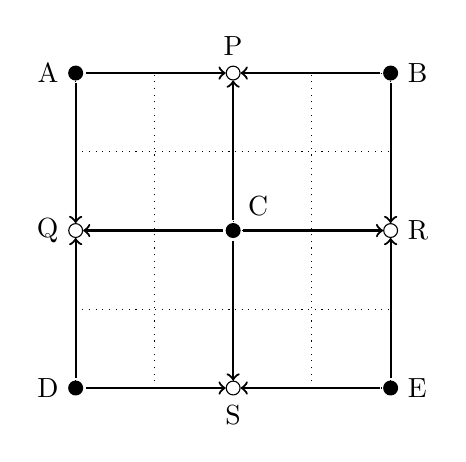
\begin{tikzpicture}[node distance=2cm]
	\draw[thin,color=black,dotted] (0,0) grid (4,4); 
	\tikzstyle{main}=[circle,fill=black,minimum size=5pt,inner sep=0pt, draw=black]
	\tikzstyle{neigh}=[circle,fill=white,minimum size=5pt,inner sep=0pt,draw=black]
	\node[main, label=left:D] 				(D) {};
	\node[neigh,right of=D, label=below:S] 	(S) {};
	\node[main, right of=S, label=right:E] 	(E) {};
	\node[neigh, above of=D, label=left:Q] 	(Q) {};
	\node[main, right of=Q, label=above right:C] 	(C) {};
	\node[neigh, right of=C, label=right:R]	(R) {};
	\node[main, above of=Q, label=left:A] 	(A) {};
	\node[neigh, right of=A, label=above:P] (P) {};
	\node[main, right of=P, label=right:B] 	(B) {};

	\begin{scope}[->, thick, shorten <=1pt] 
		\draw	(A) -> (P);
		\draw	(A) -> (Q);
		\draw	(B) -> (P);
		\draw	(B) -> (R);
		\draw	(C) -> (P);
		\draw	(C) -> (Q);
		\draw	(C) -> (R);
		\draw[label={[above]{$f(x)=x^2$}}]	(C) -> (S);
		\draw	(D) -> (Q);
		\draw	(D) -> (S);
		\draw	(E) -> (S);
		\draw	(E) -> (R);
	\end{scope}
\end{tikzpicture}
}}
\subfigure[2. iterace zahuštění]{
\label{figure:algorithm:run:iteration}
\resizebox{.48\textwidth}{!}{
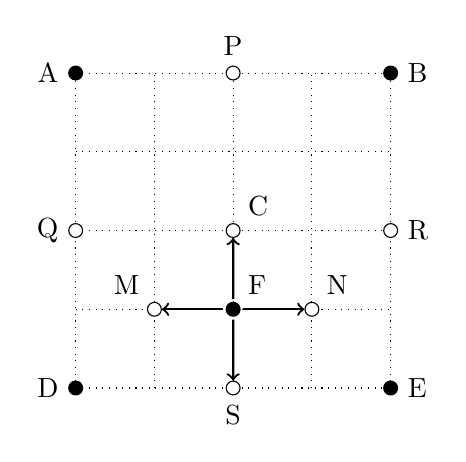
\begin{tikzpicture}[node distance=2cm]
	\draw[thin,color=black,dotted] (0,0) grid (4,4); 
	\tikzstyle{main}=[circle,fill=black,minimum size=5pt,inner sep=0pt, draw=black]
	\tikzstyle{neigh}=[circle,fill=white,minimum size=5pt,inner sep=0pt,draw=black]
	\node[main, label=left:D] 				(D) {};
	\node[neigh,right of=D, label=below:S] 	(S) {};
	\node[main, right of=S, label=right:E] 	(E) {};
	\node[neigh, above of=D, label=left:Q] 	(Q) {};
	\node[neigh, right of=Q, label=above right:C] 	(C) {};
	\node[neigh, right of=C, label=right:R]	(R) {};
	\node[main, above of=Q, label=left:A] 	(A) {};
	\node[neigh, right of=A, label=above:P] (P) {};
	\node[main, right of=P, label=right:B] 	(B) {};
	
	\node[main, label=above right:F] (F) at (2,1) {};
	\node[neigh, label=above left:M] (M) at (1,1) {};
	\node[neigh, label=above right:N] (N) at (3,1) {};
	\begin{scope}[->, thick, shorten <=1pt] 
		\draw	(F) -> (C);
		\draw	(F) -> (N);
		\draw	(F) -> (M);
		\draw	(F) -> (S);
	\end{scope}
\end{tikzpicture}
}}
\caption{Znázornění průběhu výpočtu pro dvourozměrný prostor iniciálních podmínek.
Černé tečky znázorňují hlavní a bílé pomocné body, které odpovídají bodům $\textsc{X}_{main}$ a $\textsc{X}_{neigh}$ v pseudokódu \ref{algorithm:main:original}.
Ke každému bodu $X$ odpovídá signál $s_X$. Hrana $X \rightarrow Y$ značí porovnání
$\big|\rho(\varphi, s_X)\big| \geq \rho(s_X, s_Y)$.}
\end{center}
\end{figure}

Na obrázku \ref{figure:algorithm:run:init} je ukázáno, jak vypadá iniciální zahuštění
pro dvourozměrný prostor iniciálních podmínek. Algoritmus vloží jeden hlavní bod (C) do středu prostoru. 
Tento prostřední bod obklopí dvěma vedlejšími body v každé dimenzi iniciálního prostoru (P, Q, R, S) ve vzdálenosti
poloviny velikosti prostoru v dané dimenzi. Takto vzniklé body opět obklopí dalšími, tentokrát již hlavními (A, B, D, E).
Tento postup se opakuje, dokud není prostor iniciálních podmínek dostatečně zahuštěn.
Každý z hlavních bodů s sebou během výpočtu nese odkaz na příslušné vedlejší body.
Toto iniciální zahuštění je označeno jako první iterace.

Obrázek \ref{figure:algorithm:run:iteration} znázorňuje situaci, kdy došlo k druhé iteraci zahuštění,
pro\-tože $\big|\rho(\varphi, s_C)\big| < dist(s_C, s_S)$. Ze středu úsečky CS se vytvoří
nový hlavní bod F. Pro každou dimenzi se vytvoří pomocné body tentokrát ve vzdá\-le\-nosti jedné čtvrtiny
velikosti prostoru iniciálních hodnot v dané dimenzi, tím se hlavní bod C v této
nové iteraci zahuštění stává bodem vedlejším.

V nejméně příznivém scénáři je v iteracích $0, 1, \ldots, i$ nutno pracovat s~$(2^i + 1)^d$ body,
kde $d$ je dimenze prostoru iniciálních podmínek. Algoritmus v mnoha případech
ke svému výpočtu nevyžaduje takové množství bodů. Expo\-nen\-ciál\-ní nárůst počtu
potřebných bodů se však i přesto od určité iterace za\-huš\-tě\-ní objeví. To je způsobeno
zejména regiony prostoru iniciálních podmínek, kterými prochází hranice platnosti dané formule.

Nutnost analyzovat exponenciální množství trajektorií chování společně s
výpočetní náročností numerické simulace vede k tomu, že analýza i po\-měr\-ně
malých modelů může trvat nesmírně dlouho. Tato práce se snaží tento problém řešit
distribucí výpočtu na více počítačích s využitím datového paralelismu.
